\chapter{Results}\label{chap:Results}

\section{Performance of the RRT* Algorithm}\label{sec:performanceRRT}

The goal of this master thesis in not primarily to improve the performance of the RRT* algorithm but to tune the parameters for nonlinear optimization. \newline

As mentioned in section \ref{sec:RRTstar}, the calculation time of the RRT* algorithm is mainly defined by the "rewiring" and therefore by the user-specified parameter $\gamma$ (of equation \ref{equ:ballradius}). A good straight line solution, whereas good means a short length of the straight line solution, does not necessarily lead to a good polynomial trajectory. The influence of the user specified parameter $\gamma$ on the final trajectory and the corresponding calculation time is summarized in this section. \newline
Please have in mind that a small $\gamma$ parameter means little rewiring and a large $\gamma$ parameter means lots of rewiring. The impact of the $\gamma$ parameter can be looked up in figures \ref{pic:smallGamma} and \ref{pic:smallBBX}, respectively.\newline

\begin{figure}[H]
   \centering
   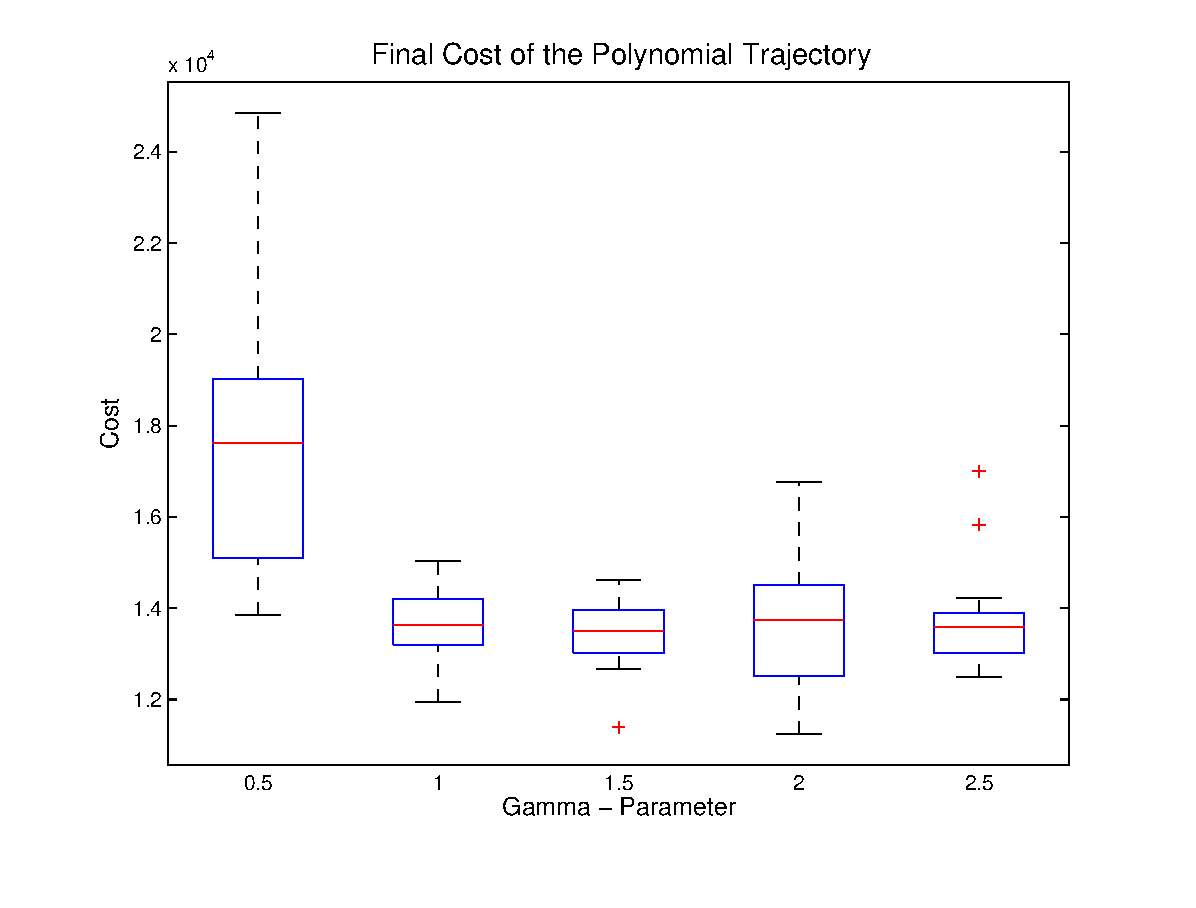
\includegraphics[trim = 14mm 10mm 15mm 0mm,clip,width=0.8\textwidth]{pics/boxplot1.eps}
   \caption{The final cost of the polynomial trajectory is depicted as a function of various $\gamma$ parameters. On each box, the red mark illustrates the median.}
   \label{pic:boxplot}
\end{figure}

Figure \ref{pic:boxplot} depicts the boxplot for different $\gamma$ parameters. Each dataset consists of 15 measurements. On each box, the central mark is the median, the edges of the box are the 25th and 75th percentiles, the whiskers extend to the most extreme
datapoints the algorithm considers to be not outliers, and the outliers are plotted individually. \newline

It becomes apparent that the small amount of rewiring associated with $\gamma = 0.5$ is too small to obtain a good polynomial trajectory. However, increasing $\gamma$ above 1 is not reducing the final trajectory cost anymore. \newline

The total computational times for the five different $\gamma$ parameters are depicted in figure \ref{pic:boxplot_time}. The total computational time is the combined duration of the RRT* algorithm and the nonlinear optimization. In contrast to the final cost, $\gamma$ parameters greater than 1 show an impact on computational time.

\begin{figure}[h]
   \centering
   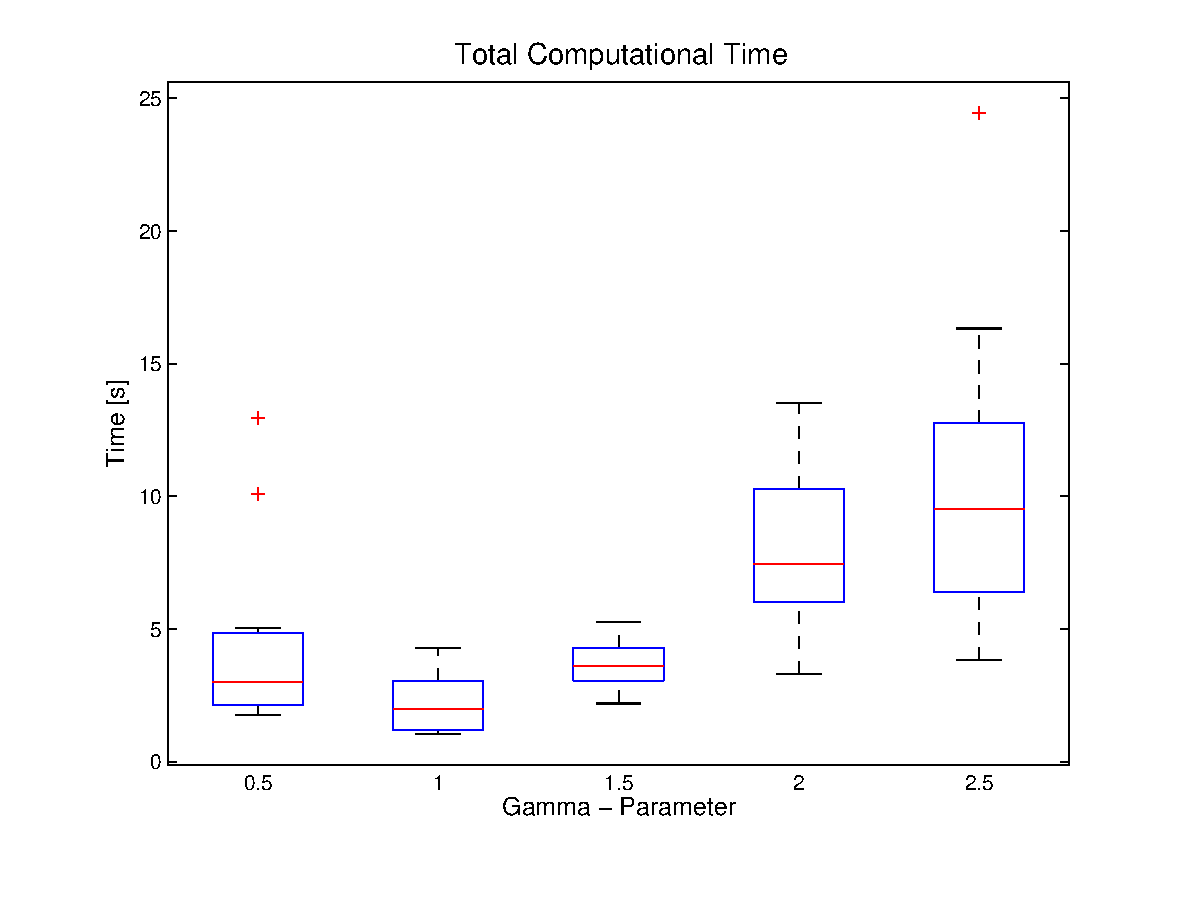
\includegraphics[trim = 14mm 10mm 15mm 0mm,clip,width=0.8\textwidth]{pics/boxplot_time.eps}
   \caption{The total computational time is depicted as a function of various $\gamma$ parameters. On each box, the red mark illustrates the median.}
   \label{pic:boxplot_time}
\end{figure}

Figure \ref{pic:boxplot_time} shows that the computational time increases significantly if $\gamma$ is larger than 1.5. This is due to the fact that the RRT* algorithm needs more time for rewiring. Furthermore, $\gamma = 0.5$ (which is not a good choice since the final cost is too high) has 2 outliers. In this 2 cases the straight line solution is not enough target-orientated and multiple vertex extensions are required to obtain a collision-free trajectory. \newline

Combining the results shown in figure \ref{pic:boxplot} and figure \ref{pic:boxplot_time}, a $\gamma$ parameter in the range of 1 to 1.5 leads to the best performance.

\section{Performance of NLopt}

To test the performance of NLopt 6 trajectories of different length were optimized. The trajectories have the same start vertex but specific goal vertices. The RRT* planning and the optimization were performed individually for each trajectory. 

Figure \ref{pic:differentGoal} depicts a start vertex and 6 different goal vertices. The figure is in bird's eye perspective and shows a crossing of different hallways. The blue cells represent the floor and the green cells represent the walls. 
In some of the hallways there are objects blocking (part of) the way. This passages are tagged with "Bottleneck". Please note that other passages may look like a bottleneck (such as the top right corner) but are not blocked. The green boxes in this passage are part of the ceiling.

\begin{figure}[H]
   \centering
   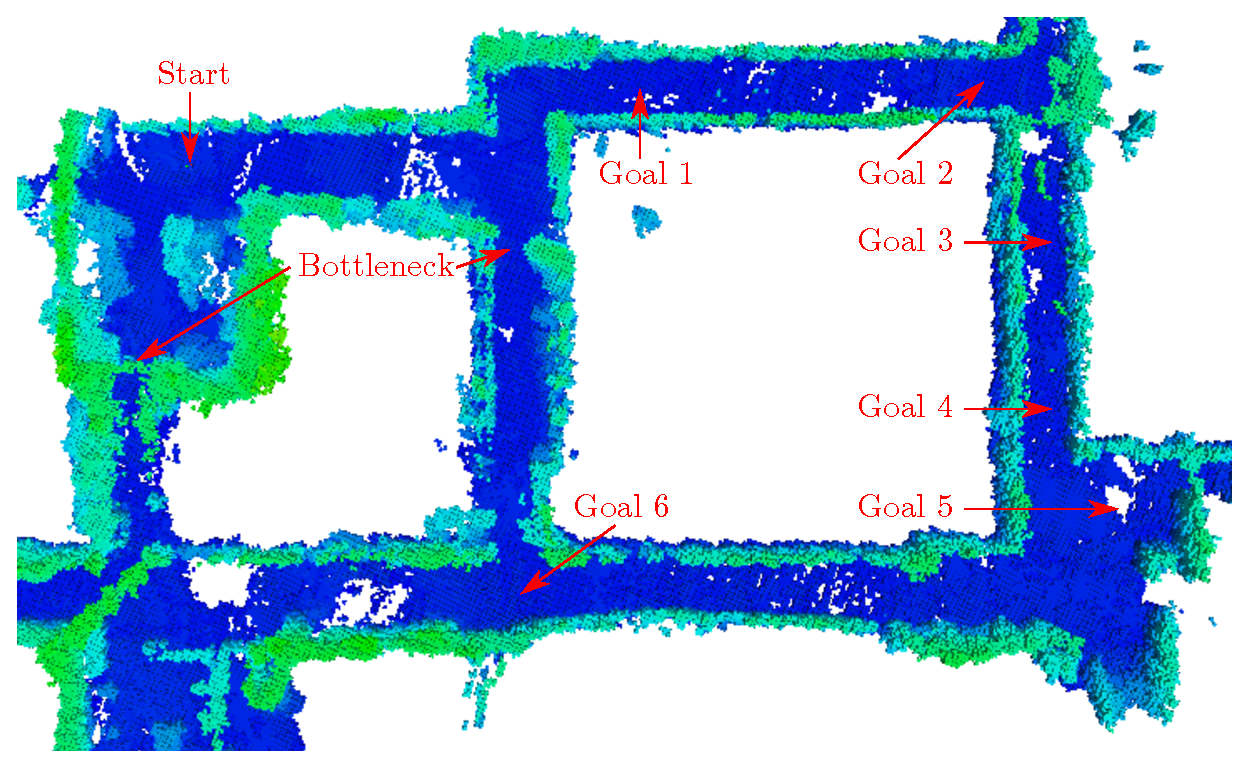
\includegraphics[trim = 14mm 15mm 17mm 0mm,clip,width=0.8\textwidth]{pics/ML4a.eps}
   \caption{Bird's eye perspective on hallways in the "ML" building of the ETH Zurich. The start vertex and 6 different goal vertices are depicted.}
   \label{pic:differentGoal}
\end{figure}

The bottleneck in the center of figure \ref{pic:differentGoal} gets significant for large bounding boxes. If the size of the bounding box is larger than $0.5m$ x $0.5m$ x $0.5m$ the trajectory is not able to pass the bottleneck anymore. Hence, a trajectory with a large bounding box has to go all the way around to proceed from the start vertex to "Goal 6" as depicted in figure \ref{pic:Goal6}.

\begin{figure}[H]
   \centering
   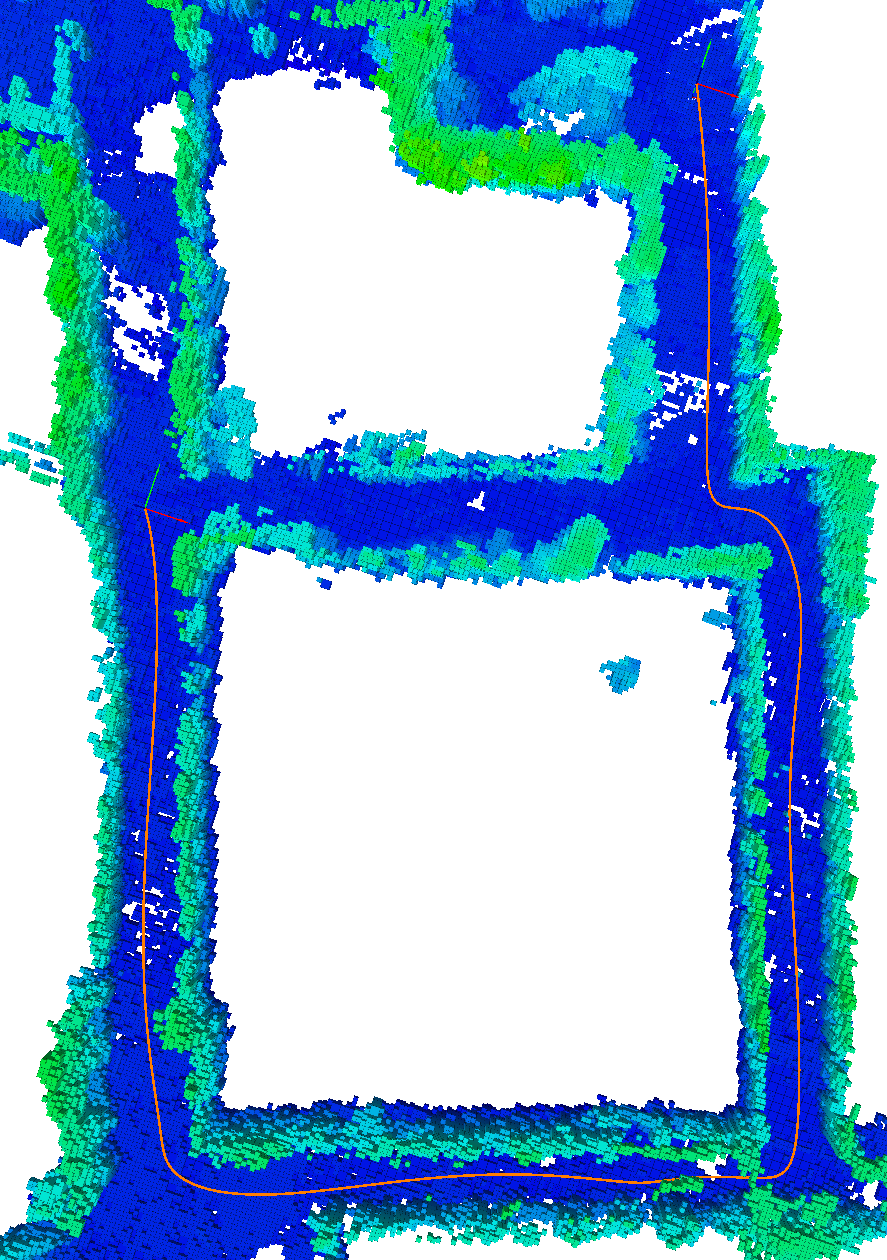
\includegraphics[angle=90,trim = 18mm 0mm 0mm 0mm,clip, width=0.8\textwidth]{pics/MapNlopt.png}
   \caption{Trajectory from the start vertex to "Goal 6". Due to the bottleneck in the hallway in the middle, the trajectory has to proceed all the way around.}
   \label{pic:Goal6}
\end{figure}

The trajectories from the start vertex to the 6 different goal vertices are examined for number of segments and the duration of NLopt. The only ending criteria for NLopt was the relative criteria on the total cost $f_{rel} = 0.02$. 
In addition to the number of segments, the number of corresponding optimization variables (endpoint derivatives $d_p$ and segment times $T_i$) are calculated. 

For all "free" vertices (which are neither the start nor the goal vertex) there are 12 optimization variables, namely the velocity, the acceleration, the jerk and the snap in the 3 dimensions. Furthermore, the segment times are optimization variables. \newline

Since the number of free vertices is the number of segment $n_{seg}$ minus 1, the equation for the number of optimization variables $n_{var}$ is:

\begin{equation}
n_{var} = (n_{seg} - 1)\cdot 12 + n_{seg}
\label{equ:numberOfSeg}
\end{equation}

The results for the 6 different goal vertices are listed in the following table:


\begin{table}[H] 
\begin{center}
    \begin{tabular}{| c | c | c | c | }
    \hline
    Goal Vertex & Segments & Optimization Variables & Optimization Time\\ \hline
   Goal 1 & 5 & 53 & $1.15s$\\ \hline
  Goal 2 & 8 & 92 & $2.94s$\\ \hline
   Goal 3 & 11 & 131 & $7.80s$\\ \hline
Goal 4 & 15 & 183& $42.96s$\\ \hline
Goal 5 & 19 & 235& $93.08s$\\ \hline
   Goal 6& 20 & 248 & $347.62s$\\
    \hline
    \end{tabular}
    \caption{The number of segments, the corresponding number of optimization variables with the respective optimization times needed by NLopt are listed.}
    \label{tab:MLoptimizationTime}
\end{center}
\end{table}

Table \ref{tab:MLoptimizationTime} shows that the optimization time (i.e. the duration of the NLopt algorithm) increases significantly for a large amount of optimization variables. Comparing the result of "Goal 5" to "Goal 6" it becomes clear, that the number of optimization variables is not the only factor which determines the optimization time. If the optimization values of the initial solution are close to the global minimum of the cost function, the optimization takes less time, and vice versa. Still, the number of optimization variables is the main factor determining the optimization. \newline

Please note that the RRT* algorithm was only executed once for every goal vertex. Due to the randomness of the RRT* algorithm, the number of segments might change for unchanged start and goal vertices.

\section{Reduction of the Optimization Variables}

The results in table \ref{tab:MLoptimizationTime} have shown that the performance of NLopt decreases with a large amount of optimization variables. In cases where the optimization time is significant (i.e. online planning) the number of optimization parameters has to be reduced. The benefits and the drawbacks of a cost function with fewer optimization variables is discussed below.

\subsection{Cost Function Without Endpoint Derivatives}

As discussed in section \ref{sec:penalty}, the minimum of the total cost function (equation \ref{equ:total_cost}) can not be found analytically but with a nonlinear optimization. \newpage

To improve readability, the total cost function is written-out again in equation \ref{equ:total_cost_Result}


\begin{equation}
J_{total} =
\begin{bmatrix}
   d_f \\
  d_p
\end{bmatrix}^T
\begin{bmatrix}
   R_{ff} & R_{fp} \\
  R_{pf} & R_{pp}
\end{bmatrix}
\begin{bmatrix}
   d_f \\
  d_p
\end{bmatrix}
+ k_T \cdot \sum_{i=1}^N T_i
\label{equ:total_cost_Result}
\end{equation}

where the optimization variables are the segment times $T_i$ and the unspecified endpoint derivatives $d_p$. $k_T$ is a user-specified weighting factor and $d_f$ is the vector containing the fixed endpoint derivatives. The 4 sub-matrices of $R$ are containing the quadratic snap rearranged according to the fixed and unspecified endpoint derivatives. \newline

In contrast to the total cost function, the geometric cost (i.e. equation \ref{equ:total_cost_Result} without the weighted sum of the segment times $T_i$) can be minimized analytically for known segment times. Therefore, the unspecified endpoint derivatives $d_p$ can be excluded from the optimization variables. In other words, in every optimization step the segment times are modified by NLopt. Then $d_p^* $ is computed according to equation \ref{equ:dpstar} with the current segment times and the total cost is calculated according to equation \ref{equ:total_cost_Result}. \newline

Since equation \ref{equ:dpstar} has to be solve every iteration once the number of optimization variables is reduced the choice of the analytical or linear solver gains in importance.

\subsection{Linear Solver}

A linear solver is able to solve a single matrix equation

\begin{equation}
A \cdot x = b
\label{equ:linearSolver}
\end{equation}

where $A$ is a matrix, $b$ a vector and $x$ is the vector containing the optimization variables. \newline

Indeed, equation \ref{equ:dpstar} is a single matrix equation which gets evident after a rearrangement of the equation:

\begin{equation}
 - R_{pp}  \cdot d_p^* =R_{fp}^T \cdot d_f
\label{equ:dpstar_Result}
\end{equation}

$d_p$  is the vector containing the optimization variables and represents $x$. $R_{fp}^T \cdot d_f$ can be taken together as vector $b$ and the matrix $-R_{pp}$ represents $A$. \newline

In this master thesis, three different techniques have been implemented to solve equation \ref{equ:dpstar_Result}.
All of them are part of "Eigen". Eigen is a C++ template library for linear algebra: matrices, vectors, numerical solvers, and related algorithms. The definition of the implemented strategies can be found on the  \href{http://eigen.tuxfamily.org/index.php?title=Main_Page}{Eigen-homepage} \cite{Eigen}:

\subsubsection{Technique 1: FullPivLU}

This class represents a $LU$ decomposition of any matrix, with complete pivoting: the matrix $A$ is decomposed as $A = PLUQ$ where $L$ is unit-lower-triangular, $U$ is upper-triangular, and $P$ and $Q$ are permutation matrices. This is a rank-revealing $LU$ decomposition. The eigenvalues (diagonal coefficients) of $U$ are sorted in such a way that any zeros are at the end. \newline

$FullPivLU$ is a very accurate technique but rather slow.

\subsubsection{Technique 2: HouseholderQR}

This class performs a $QR$ decomposition of a matrix $A$ into matrices $Q$ and $R$ such that $A = QR$ by using Householder transformations. Here, $Q$ a unitary matrix and $R$ an upper triangular matrix. The result is stored in a compact way compatible with $LAPACK$. Note that no pivoting is performed. This is not a rank-revealing decomposition.\newline

$HouseholderQR$ is a fast technique but in general less accurate than $FullPivLU$.

\subsubsection{Technique 3: Inverse}
For small fixed sizes up to $4x4$, this method uses cofactors. In the general case, this method uses class $PartialPivLU$. This class represents a $LU$ decomposition of a square invertible matrix, with partial pivoting: the matrix $A$ is decomposed as $A = PLU$ where $L$ is unit-lower-triangular, $U$ is upper-triangular, and $P$ is a permutation matrix. \newline

The performance of $Inverse$ is compared experimentally to the other techniques. \newline

First, the three techniques were tested with a long trajectory. The initial solution has been computed for a trajectory with 300 segments with random vertices. The identical set of vertices was used for all the three techniques and the results are listed in the following table:

\begin{table}[H] 
\begin{center}
    \begin{tabular}{| c | c | }
    \hline
    Technique & Computational Time  \\ \hline
  FullPivLU  & $19.52s$\\ \hline
  HouseholderQR & $3.34s$\\ \hline
 Inverse & $2.07s$\\
    \hline
    \end{tabular}
    \caption{Comparison of the three analytical solvers for a trajectory with 300 segments. Only the initial solution has been computed.}
    \label{tab:300seg}
\end{center}
\end{table}

As already mentioned, $FullPivLU$ needs considerably more computational time than $HouseholderQR$. The performance of $HouseholderQR$ and $Inverse$ are comparable.\newline

In a next step, the three techniques have been compared in the nonlinear optimization with the reduced number of optimization parameters. Meaning, the linear solver is applied every optimization step.  \newline

The RRT* algorithm was executed to find a straight line solution from the start vertex to "Goal 6" in figure \ref{pic:differentGoal}. The collision-free polynomial trajectory had 23 segments. The trajectory was optimized using $FullPivLU$ but in every iteration $HouseholderQR$ and $Inverse$ has been computed as well and the total time of the individual techniques has been stored. The optimization terminated after 883 iterations and the result of the three techniques are listed in table \ref{tab:883iter}.\newline


\begin{table}[h] 
\begin{center}
    \begin{tabular}{| c | c | }
    \hline
    Technique & Computational Time  \\ \hline
  FullPivLU  & $1.134s$\\ \hline
  HouseholderQR & $0.704s$\\ \hline
 Inverse & $0.285s$\\
    \hline
    \end{tabular}
    \caption{Comparison of the three analytical solvers for a trajectory with 23 segments. The nonlinear optimization was performed (883 iterations).}
    \label{tab:883iter}
\end{center}
\end{table}


As mentioned above $FullPivLU$ is very accurate. In the two above noted tests (and also in other performed tests) the other two techniques led to the same result as $FullPivLU$, meaning there were no numerical instability issues. This is due to the fact, that $R_{pp}$ is quadratic and a band matrix. A band matrix is a sparse matrix whose non-zero entries are confined to a diagonal band. Band matrices are beneficial from a computational point of view.


Since the numerical stability is given for all of the techniques the determining factor is the computational time. Therefore, the $Inverse$ is the preferable technique. \newline

Please note that the $FullPivLU$ and $HouseholderQR$ have to solve equation \ref{equ:dpstar} separately for each dimension. In contrast, $Inverse$ has to be computed once and can then be applied to the three dimensions. This means that $HouseholderQR$ would be faster than $Inverse$ if only one dimension had to be optimized. However, in this master thesis with three dimensions $Inverse$ can display its advantages and is applied further on. 

\subsection{Comparison of the Different Approaches}\label{sec:CompDiffApp}

Since the linear solver is now defined, the approach with the full number of optimization variables (in the interests of simplification called approach A) can be compared to the approach with the reduced number of optimization variables (approach B).\newline

Table \ref{tab:MLoptimizationTime} depicts the optimization time from the start vertex to "Goal 6" using the approach A. Table \ref{tab:883iter} depicts the computational time for the same start and goal vertex using the approach B. Caution, the time needed for the limit check $v_{max}$ and $a_{max}$ is not included in table \ref{tab:883iter}. 

Although the number of segments are slightly different (based on the randomness of RRT*) and table \ref{tab:883iter} does not include the time needed for the limit check it is obvious that approach B with a computational time of $0.285s$ is much faster than approach A with a optimization time of $347.62s$.\newline 

Now we compare the impact of the different approaches on the final trajectory cost.
As a consequence of the reduction of the optimization variables, approach B is not able to reach the global minimum of the cost function in all cases. Approach A on the other hand, is theoretically always able to reach the global minimum of the cost function. In practice, depending on the initial values and on the ending criteria, it happens that the optimization only finds a local minimum. \newline

Additionally, a third approach combining the benefits of approach A (able to reach the global minimum) and approach B (fast) is suggested. In one trajectory optimization approach B is applied in the first place and its result is than used as the initial value for approach A. This approach is called approach BA because of the chronological order. \newline

The performance of the 3 strategies has been tested experimentally.
To start with, the simple set of vertices from table \ref{tab:vertices} is reused. As depicted in figure \ref{pic:optimizedSolution}, a weighting factor of $k_T = 100$ does not lead to any values near the limitation. In this case, the global minimum of the cost function \ref{pic:optimizedSolution} can be found by only manipulating the segment times $T_i$. The endpoint derivatives $d_p$ as optimization variables are redundant. The only termination criteria for NLopt was $J_{rel} = 0.001$.



\begin{table}[H] 
\begin{center}
    \begin{tabular}{| c | c |  c |}
    \hline
    Approach & Optimization Time & Final Cost \\ \hline
  A & $1.48s$ & 944.887 \\ \hline
  B & $0.01s$ & 944.319 \\ \hline
 BA & $0.04s$ & 944.318 \\
    \hline
    \end{tabular}
    \caption{Optimization time and final cost for a trajectory with 2 segments. Weighting factor $k_T$ was set to 100 and NLopt ending criteria $J_{rel}$ was set to 0.001.}
    \label{tab:ABBA1}
\end{center}
\end{table}

As explained above, the final cost depicted in table \ref{tab:ABBA1} is (beside some numerical differences) the same for the three approaches. Approach B is the fastest and approach A is by fare the slowest. \newline

Now the weighting factor $k_T$ is increased to 2000 (corresponding to figure \ref{pic:optimizedSolution2k2000}). This  aggressive trajectory stays at the velocity limit for a certain time. Due to that, the segment times $T_i$ are no longer sufficient to reach the global minimum of the cost function.

\begin{table}[H] 
\begin{center}
    \begin{tabular}{| c | c |  c |}
    \hline
    Approach & Optimization Time & Final Cost \\ \hline
  A & $0.17s$ & 15295.9 \\ \hline
  B & $0.02s$ &  15994.5\\ \hline
 BA & $0.12s$ &  15047.9\\
    \hline
    \end{tabular}
    \caption{Optimization time and final cost for a trajectory with 2 segments. Weighting factor $k_T$ was set to 2000 and NLopt ending criteria $J_{rel}$ was set to 0.001.}
    \label{tab:ABBA2}
\end{center}
\end{table}

As can be seen in table \ref{tab:ABBA2}, approach B is again the fastest one. Due to the velocity limitation, approach B is not able to reach the global minimum of the cost function. Comparing the cost of approach A (which could theoretically reach the global minimum) and approach BA, is seems surprising that approach A could not find a trajectory as good as approach BA did. The reason is that approach A got stuck in a local minimum. \newline

But how could approach BA overcome this local minimum? Part A of approach BA only starts as soon as part B is terminated. Therefore, the initial values for part A are closer to the global minimum and the estimation of the initial step size for NLopt is improved. Both factors lead to a better overall performance of the NLopt algorithm and approach BA can find the best trajectory. \newline

Summarizing, table \ref{tab:MLoptimizationTime} shows that approach A is very slow if the number of segments is high. In addition, approach BA performs better in terms of final cost as can be seen in table \ref{tab:ABBA2}. Taken together, approach A is the approach with the worst performance and is not used any longer.\newline

So far, approach B and approach BA have been compared for a trajectory with 2 segments. In a next step, approach BA was used to find a trajectory from the start vertex to "Goal 1" in figure \ref{pic:differentGoal}. For 5 iterations, the number of segments fluctuated between 6 and 9, i.e. between 66 and 105 optimization variables for approach A. The parameters for this examination were: $\gamma = 1$, $J_{rel} = 0.02$ and $k_T = 5000$. A high $k_T$ guaranties that the limitation on velocity/acceleration are called into action. Otherwise, part B would have no effect at all. The optimization times for both parts are measured individually, i.e. optimization time A is the additional time after part B.

\begin{table}[H] 
\begin{center}
    \begin{tabular}{| c | c | c |  c | c |}
    \hline
   Segments  & Opt. Time B & Final Cost B & Opt. Time A & Final Cost A \\ \hline
 7& $0.54s$ & 51577.7 & $2.79s$ & 51575 \\ \hline
 6& $0.09s$ & 54142.9 & $1.72s$ & 53917.5 \\ \hline
 9& $0.38s$ &56145.4  & $8.53s$ & 56129.6 \\ \hline
 7& $0.49s$ & 57110.4 & $1.47s$ & 57104.4 \\ \hline
 6& $0.03s$ & 56020.7  & $1.76s$ & 55553.2\\
    \hline
    \end{tabular}
    \caption{Multiple trajectories from start to "Goal 1". Parameters were: $\gamma = 1$, $J_{rel} = 0.02$ and $k_T = 5000$.}
    \label{tab:BA_compare}
\end{center}
\end{table}

Apparent from table \ref{tab:BA_compare}, the benefit of connecting part A in series with part B is little. Furthermore, part B (and therefore approach B) is much faster than part A. \newline

As a consequence, approach B has the best overall performance. Approach BA only makes sense if a trajectory with little segments has to be optimized to its  limits.

















